\documentclass[12pt]{beamer}

\usepackage[utf8]{inputenc}
\usepackage{amsmath}
\usepackage{hyperref}
\usepackage{graphicx}
\usepackage{caption}
\usepackage{subcaption}
\usepackage[style=ext-authoryear, backend=biber]{biblatex}
\addbibresource{refs.bib}

\DeclareOuterCiteDelims{parencite}{\bibopenbracket}{\bibclosebracket}

\begin{document}
\begin{frame}{Objective-Function Learning in Electricity Market~\parencite{objective_function_meta}}
  \begin{itemize}
    \item Target: bidding behavior modeled by objective/reward function
    \item standard feed-forward NN as objective function
    \pause
    \item agent: electricity generator
    \item state: price, electricity capacity/amount, forecast demand
    \item action: bid in market (comprised of price and capacity)
  \end{itemize}
\end{frame}

\begin{frame}{Results from \parencite{objective_function_meta}}
  \begin{figure}[h!]
    \begin{subfigure}{0.4\textwidth}
      \centering
      \begin{subfigure}{\textwidth}
        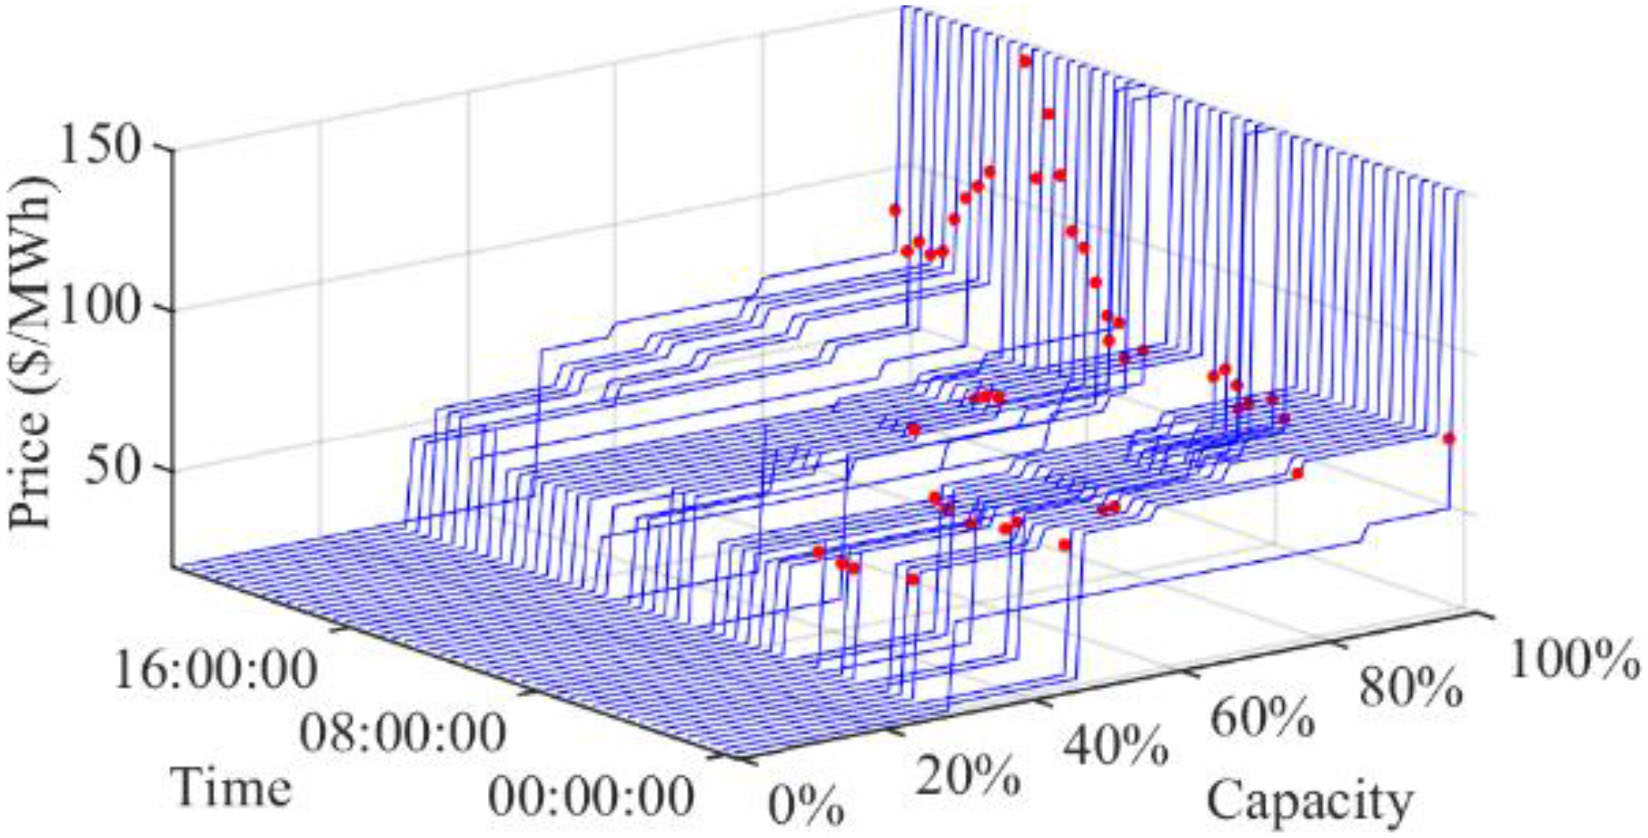
\includegraphics[width=0.95\textwidth]{./identified_vs_assumed_01_1.png}
        \caption{Inverse RL reward function for ER04}
      \end{subfigure}
      \begin{subfigure}{\textwidth}
        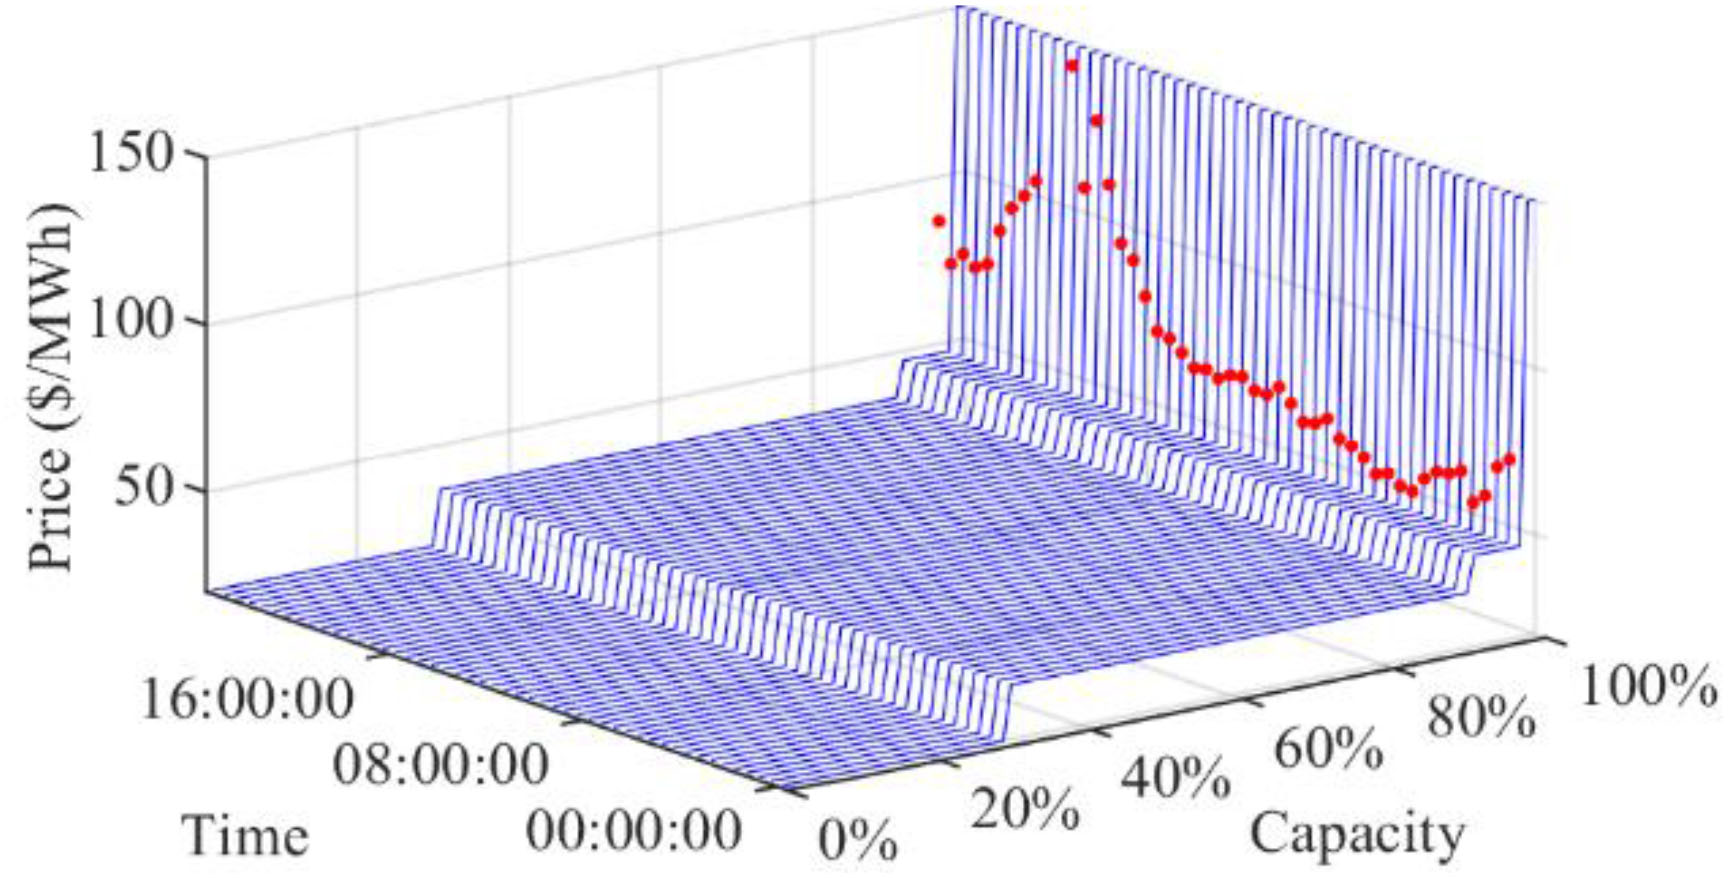
\includegraphics[width=0.95\textwidth]{./identified_vs_assumed_01_2.png}
        \caption{Assumed reward function for ER04}
      \end{subfigure}
    \end{subfigure}%
    \begin{subfigure}{0.4\textwidth}
      \centering
      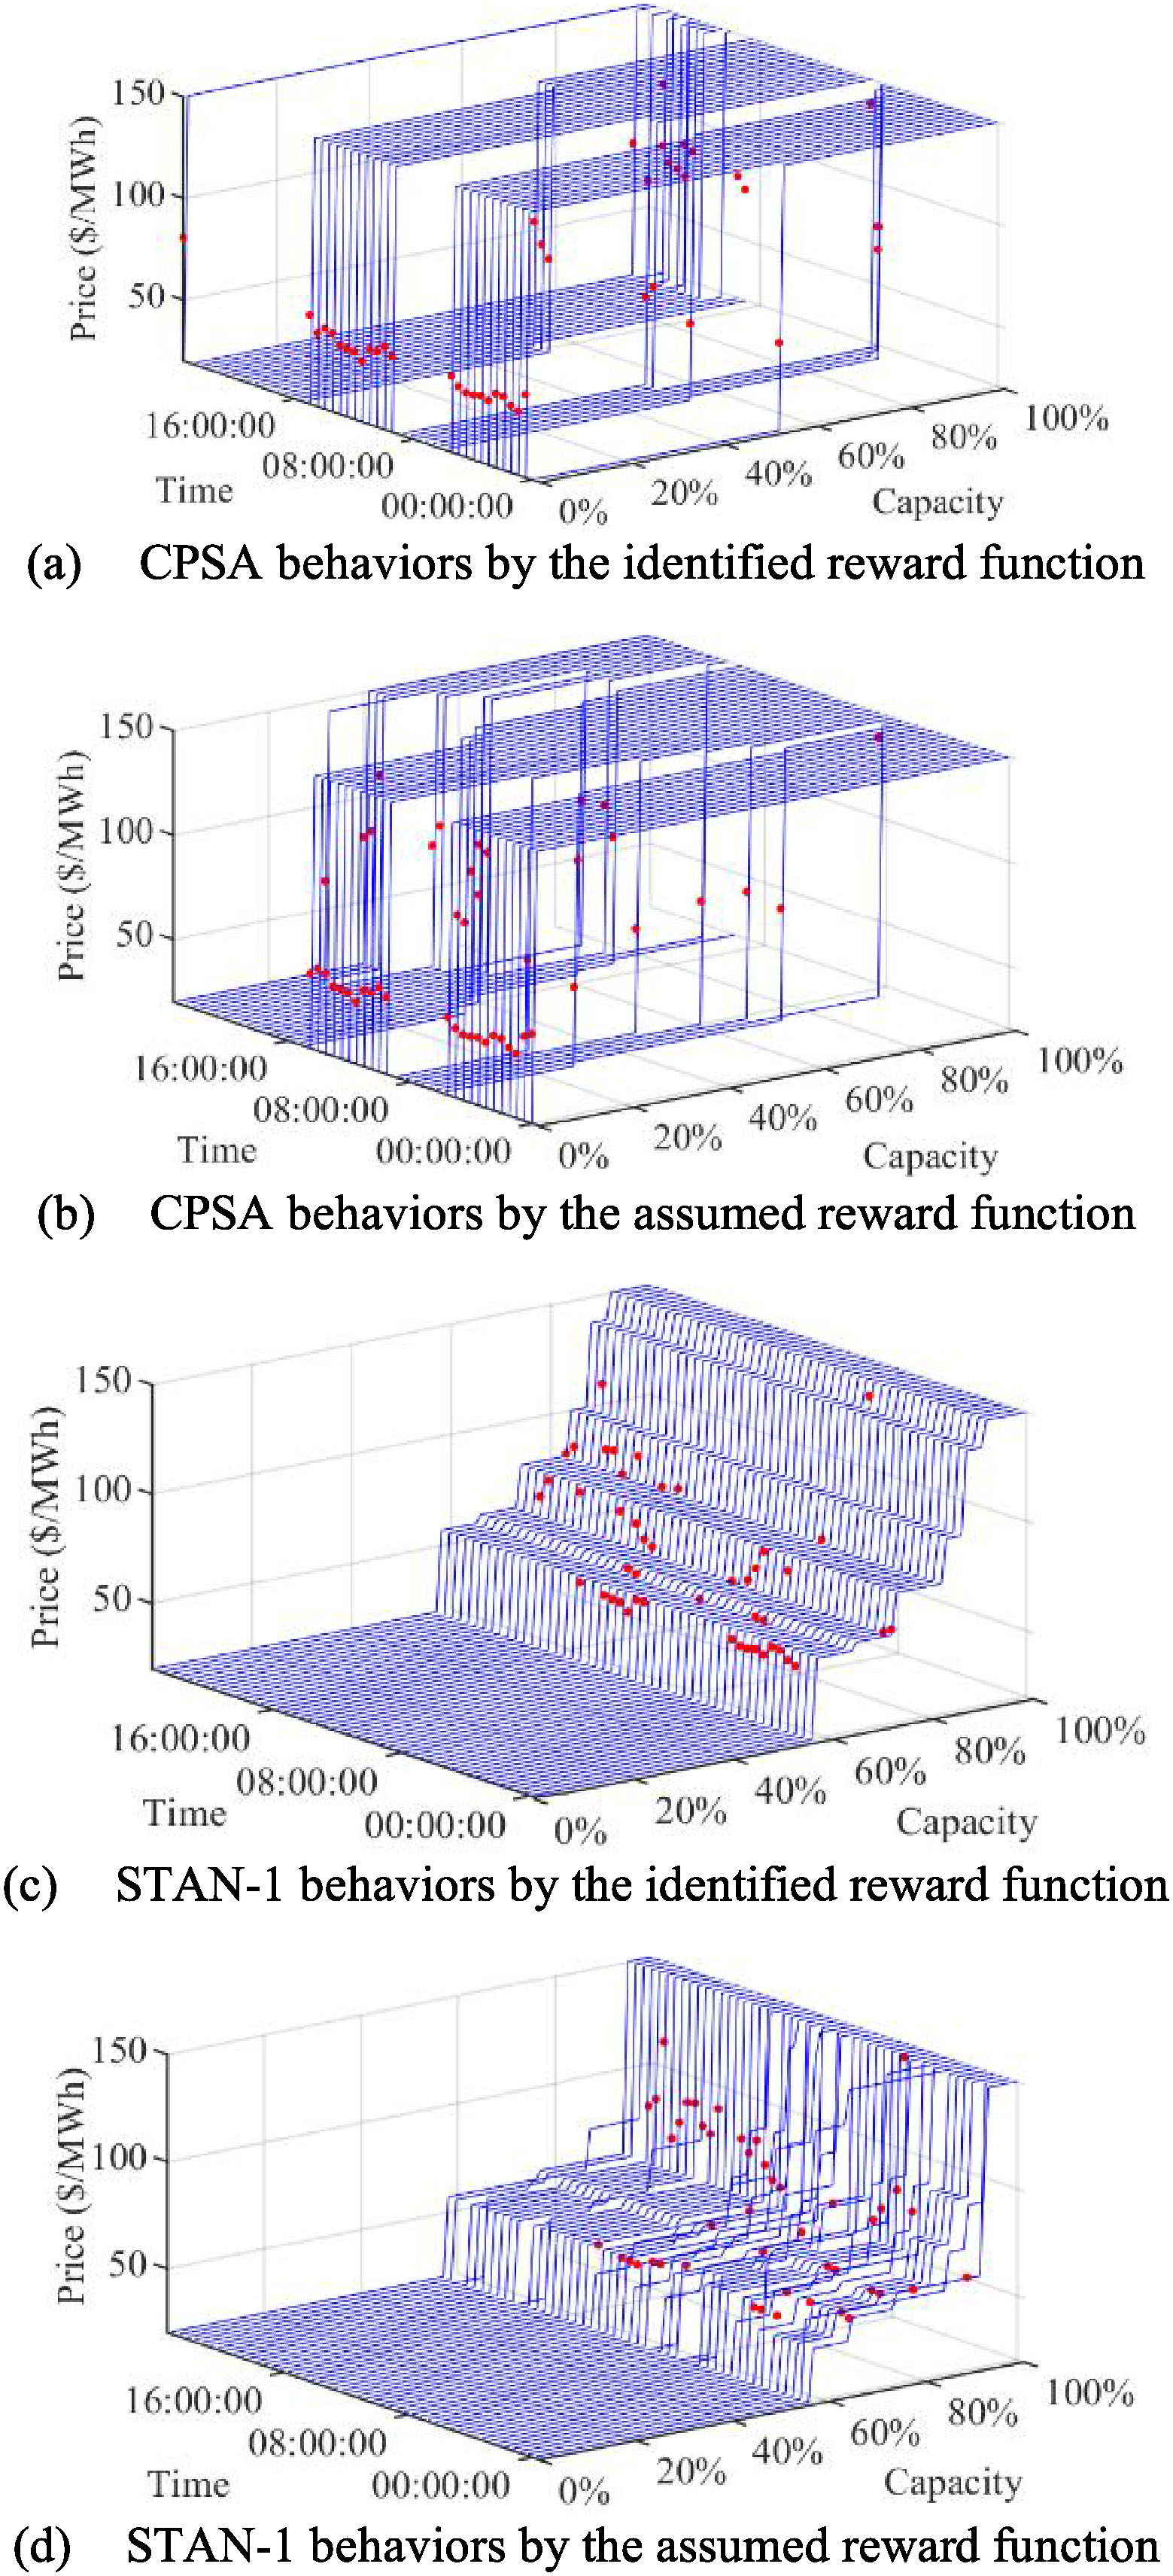
\includegraphics[height=0.8\textheight,width=0.8\textwidth]{./identified_vs_assumed_02.png}
    \end{subfigure}%
  \end{figure}
\end{frame}

\end{document}
